\subsection{一个广群、一个幺半群、一个群的代数}

回忆一下，广群是带有一个合成律的集合（I，§ 1，第 1 号）。设 S 是一个以乘法记号书写的广群，令 \(\mathbf{E} = \mathbf{A}^{(\mathbb{S})}\) 为 S 中元素的形式线性组合构成的 A-模（II，§ 1，第 11 号）；我们知道有一个典范映射 \(s \mapsto e_s\) （由 S 到 \(\mathbf{A}^{(\mathbb{S})}\) 中），使得族 \((e_s)_{s \in \mathbb{S}}\) 是 \(\mathbf{A}^{(\mathbb{S})}\) 的基（称为典范基），于是 \(\mathbf{A}^{(\mathbb{S})}\) 的每个元素都可唯一地写成 \(\sum_{s \in \mathbb{S}} \alpha_s e_s\) 的形式，其中 \((\alpha_s)\) 是 A 的元素的有限支集族。则在 E 上定义一个 A-代数结构，其方法是把典范基的乘法表取为

\[
e _ {s} e _ {t} = e _ {s t}\tag{35}
\]

这样定义的代数 E 称为广群 S 在 A 上的代数。若 \(x = \sum_{s \in S} \xi_{s} e_{s}\) 与 \(y = \sum_{s \in S} \eta_{s} e_{s}\) 是 E 的两个元素，则

\[
x y = \sum_ {s \in \mathbb {S}} \left(\sum_ {t u = s} \xi_ {t} \eta_ {u}\right) e _ {s}.
\]

当 S 是幺半群（相应地，群）时，E 称为 S 在 A 上的幺半群（相应地，群）代数；此时它是一个结合代数（§ 1，第 7 号）；类似地，当 S 是交换幺半群时，其代数是结合的且交换的。最后，若广群 S 具有单位元 \(u\) ，则 \(e_u\) 是代数 E 的单位元；由于元素 \(e_u\) 是自由的，A 于是与 E 的子代数 \(Ae_u\) 等同。

当 \(A \neq \{0\}\) 时，S 有时被等同于它在单射 \(s \mapsto e_{s}\) 下的像，于是 E 的元素可写成 \(\sum_{s \in S} \alpha_{s}s\) ；但当 S 以加法记号书写时，这一等同（若不引起混淆）是不可能的。这时也常以 \(e^{s}\) 代替 \(e_{s}\) 来写。

设 B 是另一个交换环， \(\rho: A \to B\) 是一个环同态；考虑同一广群 S 在 A 上与 B 上的代数 \(E = A^{(S)}\) 与 \(E' = B^{(S)}\) ，并令 \((e_s)_{s \in S}\) 与 \((e_s')_{s \in S}\) 分别为它们的典范基。代数 \(B^{(S)}\) 在 A-线性映射 \(j\) （它使得 \(j(e_s \otimes 1) = e_s'\) 对所有 \(s \in S\) 成立）下典范地等同于代数 \(A^{(S)} \otimes_A B\) ——它由 \(A^{(S)}\) 把标量环扩张到 B 而得到——（II，§ 1，第 11 号，命题 17 的推论 3）。

命题 6. 设 S 为一个广群，F 为一个 A-代数，且 f 为一个同态，它把

S 映入仅带乘法结构的 F。则存在且仅存在一个 A-代数同态 \(\bar{f}:\mathbf{A}^{(\mathbb{S})}\to\mathbf{F}\) 使图表交换

\begin{enumerate}
\def\labelenumi{(\arabic{enumi})}
\setcounter{enumi}{35}
\tightlist
\item
\end{enumerate}

\pandocbounded{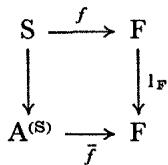
\includegraphics[keepaspectratio]{images/part003_a94682a2.jpg}}

（其中左边的竖直箭头是典范映射 \(s \mapsto e_s\) ）。

设 \(\bar{f}:\mathbf{A}^{(\mathrm{S})}\to\mathbf{F}\) 是唯一的 A-模同态，使得 \(\bar{f}(e_{s})=\bar{f}(s)\) （II，§ 1，第 11 号，命题 17 的推论 3）；只需验证 \(\bar{f}\) 是代数同态，而为此只需证明 \(\bar{f}(e_{s}e_{t})=\bar{f}(e_{s})\bar{f}(e_{t})\) ，它由定义与假设 \(f(st)=f(s)f(t)\) 直接得出。

命题 6 表达了如下事实：由 \(\mathbf{A}^{(\mathbb{S})}\) 与典范映射 \(s\mapsto e_s\) 组成的有序对是泛映射问题（《集合论》，IV，§ 3，第 1 号）的一个解，其中 \(\Sigma\) 是 A-代数结构这一种类，而 \(\alpha\) 映射是把 S 映入一个仅带其乘法律的 A-代数的同态。

推论。设 S, S' 为两个广群， \(g:S\to S'\) 为一个同态。则存在且仅存在一个 A-代数同态 \(u:A^{(S)}\to A^{(S')}\) 使图表交换

\pandocbounded{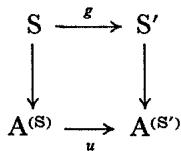
\includegraphics[keepaspectratio]{images/part003_71823134.jpg}}

（其中竖直箭头是典范映射）。

只需把命题 6 应用于取 \(f\) 为复合映射 \(\mathbf{S} \xrightarrow{g} \mathbf{S}' \to \mathbf{A}^{(\mathbf{S}')}\) 的情形。

特别地，若 T 是广群 S（I，§ 1，第 4 号）的稳定子集，则形如 \(\sum_{s\in\mathbf{T}}\alpha_s e_s\) 的元素（属于 \(\mathbf{A}^{(\mathbf{S})}\) ）所成的集合是 \(\mathbf{A}^{(\mathbf{S})}\) 的一个子代数，它典范同构于代数 \(\mathbf{A}^{(\mathbf{T})}\) ，且有时与后者等同。

例。设 V 是一个 A-模，S 是一个在 V 上从左边作用的幺半群；这就是说（I，§ 5，第 1 号），给定了一个映射 \((s, x) \mapsto s.x\) （由 S 到 V），使得 \(s.(x + y) = s.x + s.y\) , \(s.(\alpha x) = \alpha(s.x)\) 与 \(s.(t.x) = (st).x\) 对 \(s, t\) （在 S 中）、 \(x, y\) （在 V 中）与 \(\alpha \in \mathbf{A}\) 成立，且（把 \(e\) 记作 S 的单位元）对 \(x \in V\) 有 e.x = x。写 \(f(s)(x) = s.x\) ，则 f 是 S 到代数 \(\operatorname{End}_{\mathbf{A}}(\mathbf{V})\) （仅带其乘法律）中的一个同态，它把单位元 e 映到单位元 \(1_{V}\) 。应用命题 6，得到一个 A-代数同态 \(\bar{f}: \mathbf{A}^{(\mathbf{S})} \to \operatorname{End}_{\mathbf{A}}(\mathbf{V})\) ，它给出 V 的底群在 \(\mathbf{A}^{(\mathbf{S})}\) 上的一个左模结构。

这使我们能把带算子的交换群的研究归结为模的研究。因为设 M 是一个带算子的交换群，其运算以加法书写，所有外部律以乘法书写。设 \(\Omega\) 为 M 上各个外部律的算子定义域的和集（《集合论》，II，§ 4，第 8 号），其中每个定义域都被典范地等同于 \(\Omega\) 的一个子集。设 \(\mathrm{Mo}(\Omega)\) 为在 \(\Omega\) 上构造的自由幺半群（I，§ 7，第 2 号）；一个作用律

\[
(s, x) \mapsto s. x
\]

在 M 上定义，以 \(\mathrm{Mo}(\Omega)\) 为算子域，通过对 \(\mathrm{Mo}(\Omega)\) 中字 s 的长度作归纳来定义；若 s 的长度为 0，则它是空字 e，我们对所有 \(x \in M\) 写 e.x = x。若 x 的长度为 \(n \geqslant 1\) ，则它可以唯一地写成 s = tu，其中 u 的长度为 n - 1，t 的长度为 1，因此 \(t \in \Omega\) ；随后我们写 s.x = t.(u.x)。对任意两个字 s 与 \(s'\) （在 \(\mathrm{Mo}(\Omega)\) 中），关系 \(s.(s'.x) = (ss').x\) 通过对 s 的长度作归纳来验证。

然后应用上述方法，就在 M 上得到一个左 \(\mathbf{Z}^{(\mathrm{Mo}(\Omega))}\) -模结构，并且不难验证，带算子群论中的通常概念（稳定子群、同态）对带算子的交换群与这样关联于它们的模来说是相同的。

